% Preamble
\documentclass[12pt, a4paper]{article}
\title{Things to do \\\emph{After}\\Installing Arch Linux}
\author{Written by Volunteers}
\date{July 10, 2021}

% Packages
\usepackage{graphicx}
\graphicspath{{images/}}
\usepackage{xcolor}
\usepackage{caption}

% Body
\begin{document}
\maketitle

\begin{huge}
\begin{enumerate}
	\item \emph{Audio}
	\item \emph{Appearance}
	\item \emph{Fonts}
	\item \emph{Printer}
\end{enumerate}
\end{huge}

\newpage
\section{Audio}
\paragraph{}
First of all you need to install \emph{alsa-utils} package.
\begin{flushleft}
	\$ sudo pacman -S alsa-utils
\end{flushleft}
\paragraph{}
Then all you have to do is to type alsamixer in terminal and change the value of "\textcolor{red}{Master}".\\
\begin{center}
	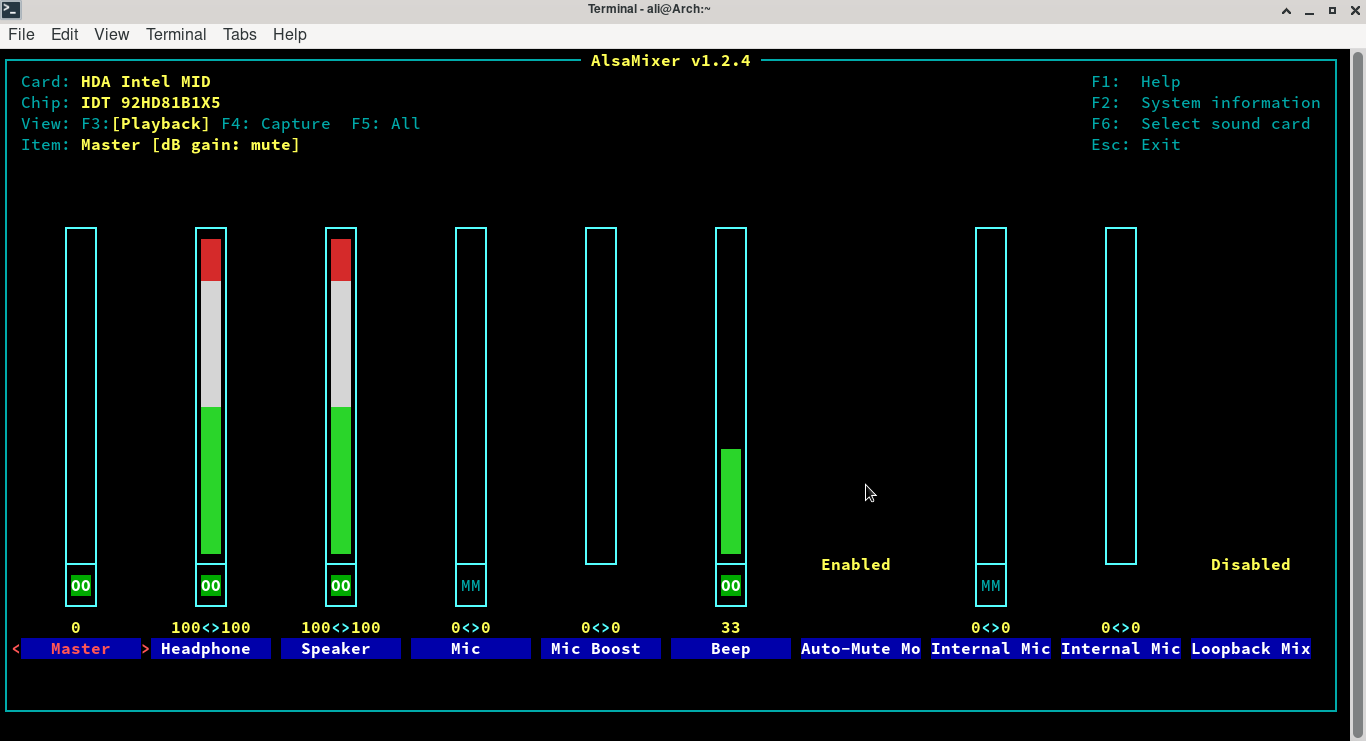
\includegraphics[scale=0.3]{mute.png}
	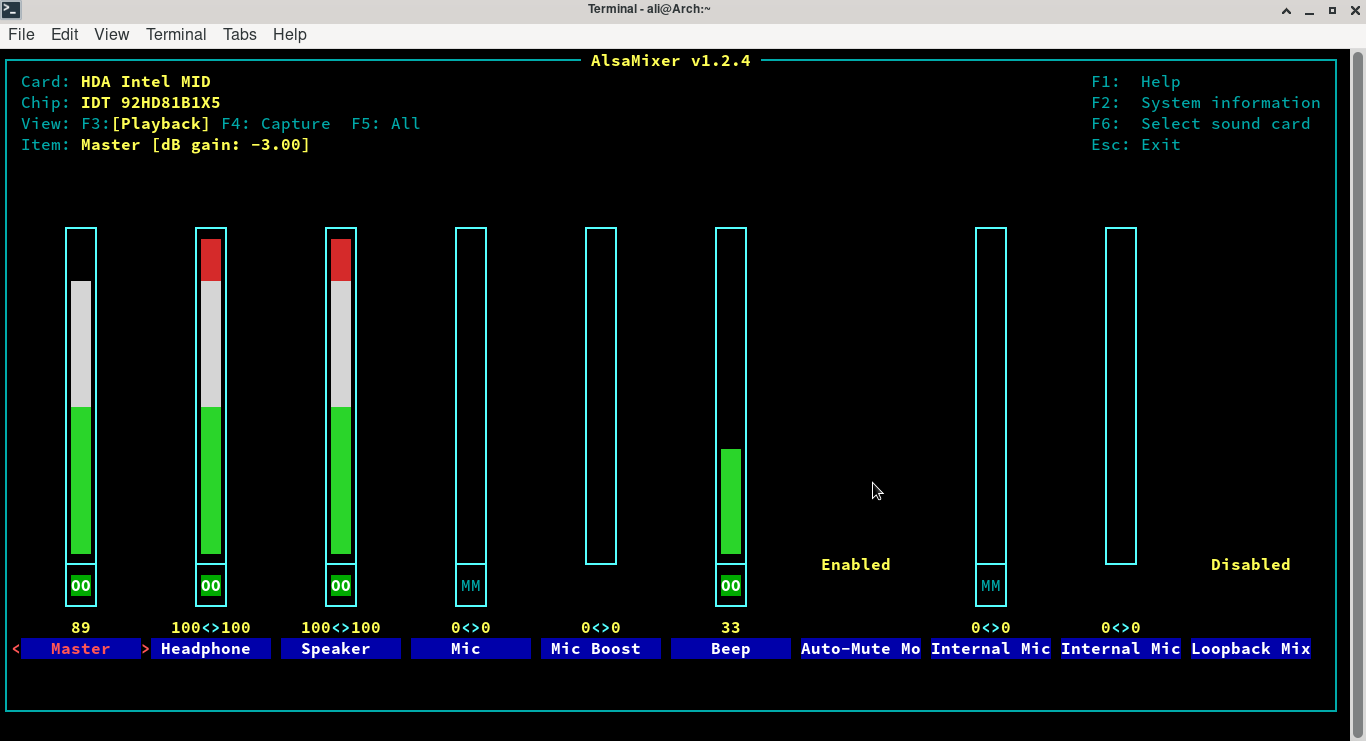
\includegraphics[scale=0.3]{audio.png}
\end{center}

\paragraph{}
You can also set \emph{Shortcuts} (Hotkeys) with amixer.
\par amixer set Master +2
\par amixer set Master -2
\par amixer set Mute 

\begin{center}
	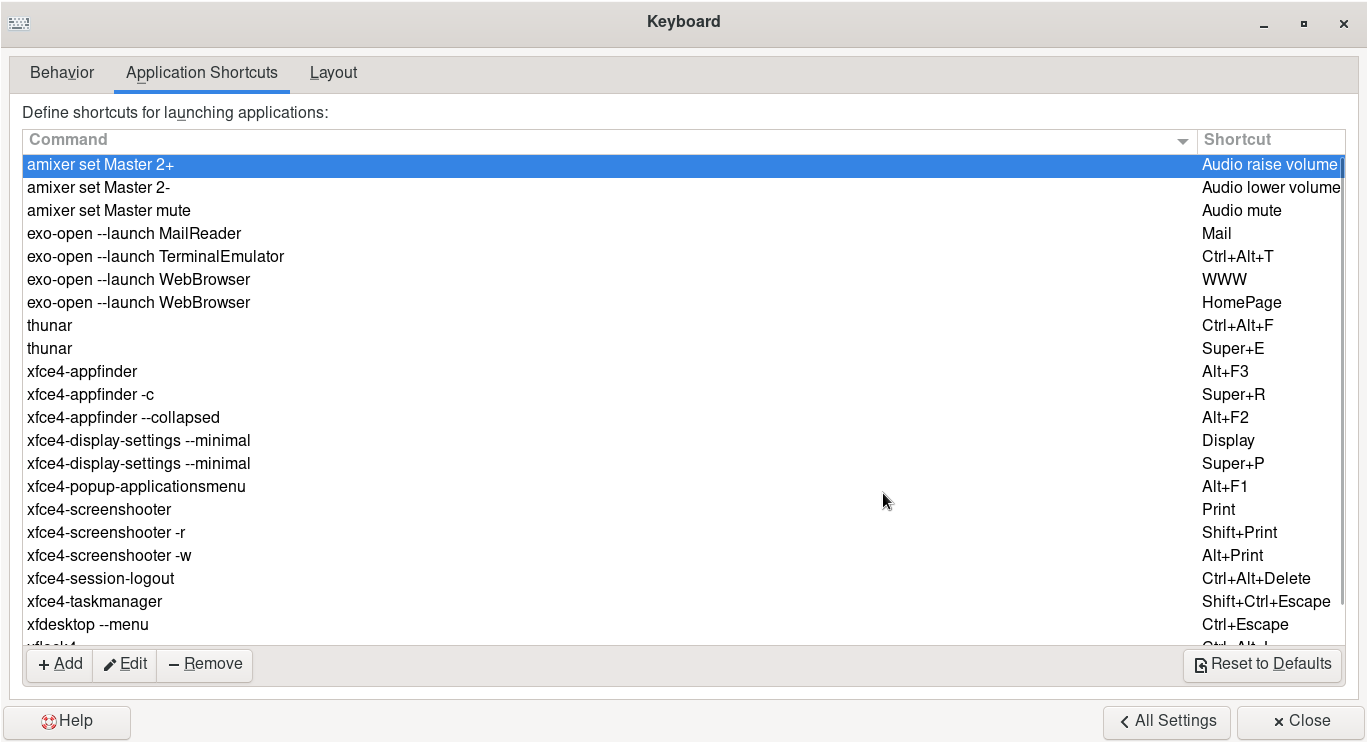
\includegraphics[scale=0.3]{amixer.png}
\end{center}

\begin{large}
\par Now you can easily change your \emph{"Audio Volume"} by any key that you selected for these options.\\
\par I recommend to install \emph{"pulseaudio"} for better experience.\\
\end{large}

\begin{center}
	\begin{tabular}{|c|}\hline
		This is for xfce4 desktop environment :\\ \hline
		\# pacman -S pulseaudio xfce4-pulseaudio-plugin\\ \hline
		\$ pulseaudio $--$start\\
		\hline \\
		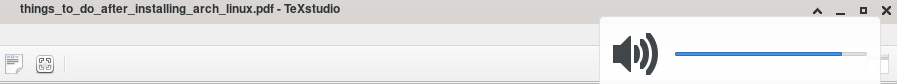
\includegraphics[scale=0.5]{pulseaudio.png}\\
		\hline
	\end{tabular}
\end{center}

\newpage
\section{Appearance}
\paragraph{}
First of all install theme \& icon.

\begin{center}
	\begin{tabular}{|c|} \hline
	\$ sudo pacman -S adapta$-$gtk$-$theme papirus$-$icon$-$theme\\ \hline
	\end{tabular}
\end{center}


\begin{large}
 \paragraph{}
 Then change your window manager \& appearance settings :
 
 \section*{Window Manager > Style}
 \paragraph{}
 select \emph{Adapta$-$Nokto} as your \emph{Style}. 
 
 \section*{Appearance > Style}
 \paragraph{}
 select \emph{Adapta$-$Nokto$-$Eta} as your \emph{Style}.
 
 \section*{Appearance > Icons}
 \paragraph{}
 select \emph{Papirus$-$Dark} as your \emph{Icon}.\\
 
 \centering
 \begin{tabular}{|c|} \hline
 	\$ reboot\\ \hline
 \end{tabular}
 
\end{large}

\newpage
\section{Fonts}
\paragraph{}
You can easily install \emph{fonts} for \emph{Arch Linux}. First of all you need to \emph{download} the font files. Then use \emph{"mv"} command or you file manager to store \emph{.ttf} files in a specific directory.\\

\begin{large}
\begin{center}
	\begin{tabular}{|c|} \hline
\# pacman -S zip unzip noto$-$fonts$-$emoji\\ \hline
\$ mkdir $\sim$/.fonts\\ \hline
\$ cd /tmp\\ \hline
\$ wget [File-URL]\\ \hline
\$ unzip *zip\\ \hline
\$ mv *ttf -t $\sim$/.fonts\\ \hline
\$ fc-cache -fv\\ \hline
	\end{tabular}
\end{center}
\end{large}

\section*{Notes :}
\paragraph{}
I read an article about fonts which said it seems the \emph{$\sim$/.fonts} is deprecated. So i recommend you to replace \emph{$\sim$/.fonts} with \emph{$\sim$/.local/share/fonts} directory.

\paragraph{}
With \emph{fc-list} command you can see the list of fonts installed on your home.
\paragraph{}
Finally make an XML file like this one :
\begin{center}
	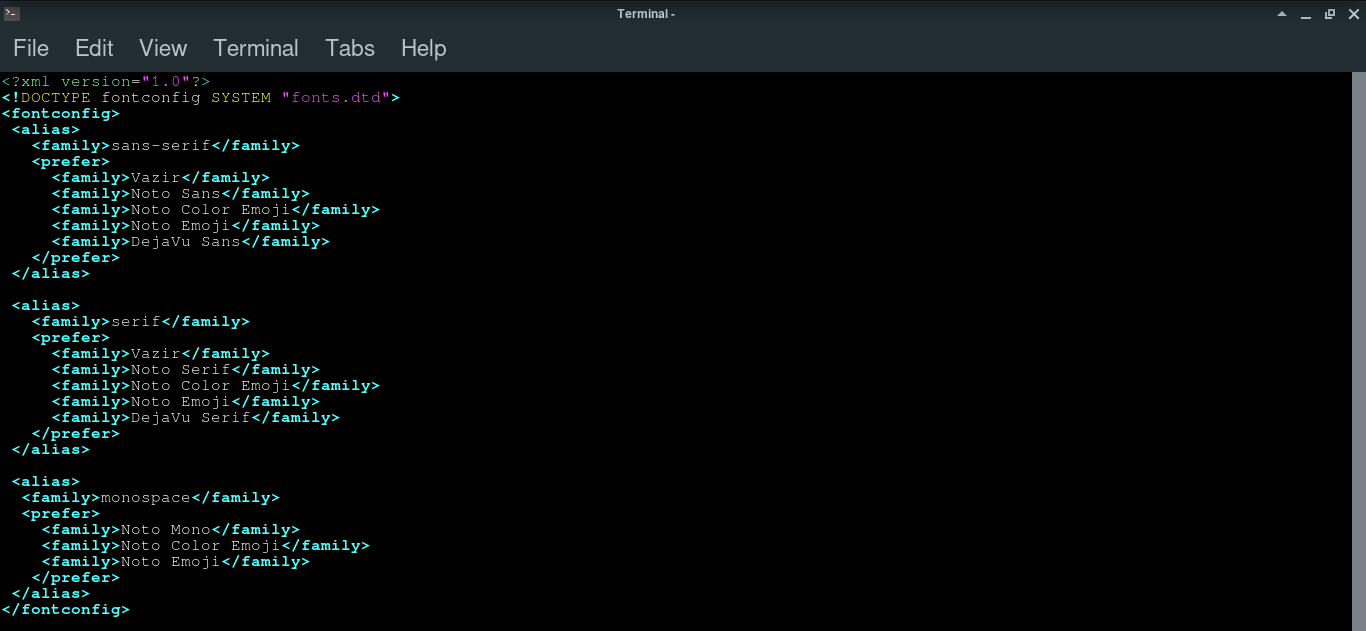
\includegraphics[scale=0.25]{fontconfig}
	fonts.conf
\end{center}

\section{Printer}
\paragraph{}
You can easily install your Printer driver. Just install cups \& splix (for \emph{samsung} printers) and add your printer to cups.\\
\# pacman -S cups splix\\
\par in your browser type "localhost:631" and follow these instructions to add your printer to cups :\\

\begin{large}
	\captionsetup[figure]{labelformat=empty}
	\begin{figure}[h!]
		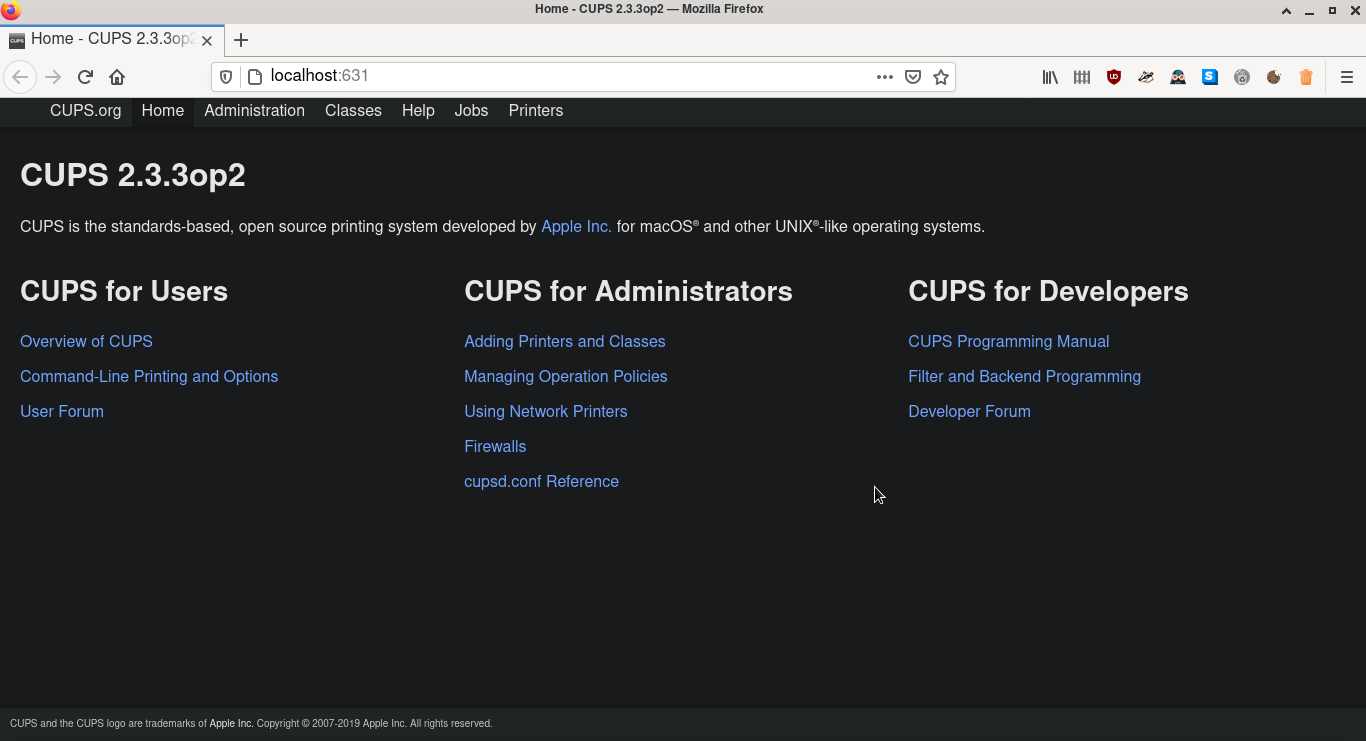
\includegraphics[scale=0.22]{cups-1}
		\caption{\emph{Cups Menu}}
	\end{figure}
\end{large}

\begin{large}
	Select \emph{"Administration"}.
	\captionsetup[figure]{labelformat=empty}
	\begin{figure}[h!]
		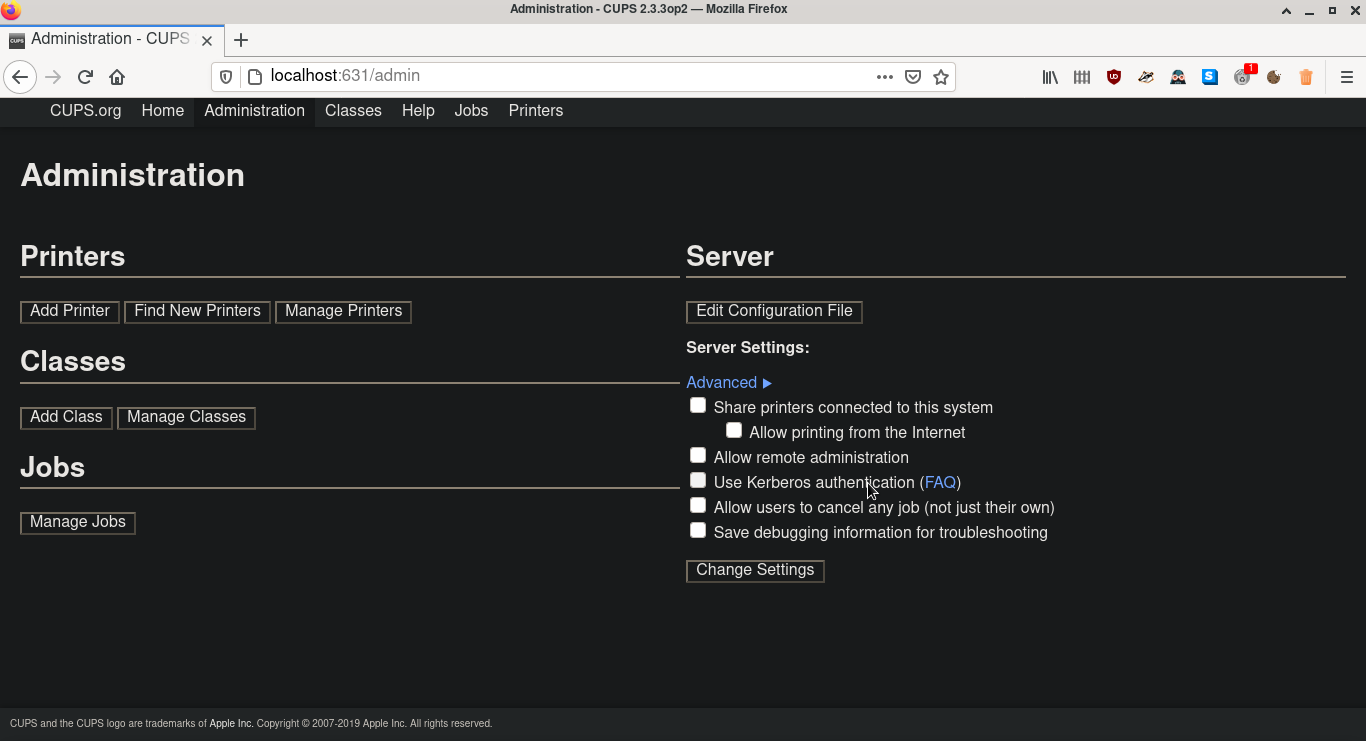
\includegraphics[scale=0.22]{cups-2}
		\caption{\emph{Administration Menu}}
	\end{figure}
\end{large}

\begin{large}
	Select \emph{"Add Printer"} and \emph{login} as \textbf{root}.\\
	\par Finally find your \emph{printer model} and save changes.
	\captionsetup[figure]{labelformat=empty}
	\begin{figure}[h!]
		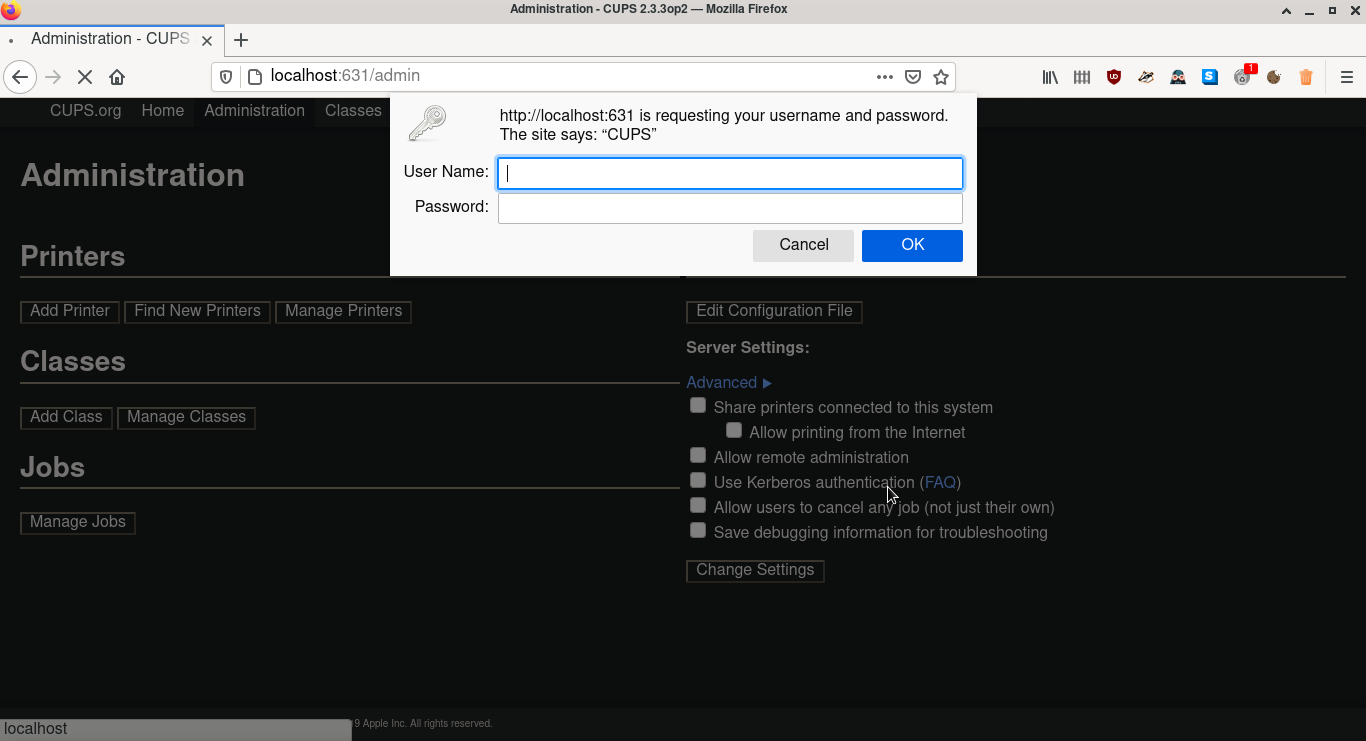
\includegraphics[scale=0.25]{cups-3}
		\caption{\emph{Add Printer}}
	\end{figure}
\end{large}
\end{document}
